
\section{Network Flow Models and Applications}

Network flow models are used to optimize the movement of commodities, resources, or information through a network while satisfying capacity and demand constraints. These models have a broad range of applications in various fields:

\begin{itemize}
    \item \textbf{Transportation and Logistics}: Optimizing the movement of goods through a supply chain while minimizing transportation costs.
    \item \textbf{Telecommunications}: Managing data traffic flow in networks to minimize congestion and latency.
    \item \textbf{Water and Energy Distribution}: Balancing water flow in pipeline systems or optimizing power grid distribution to minimize energy loss.
    \item \textbf{Project Scheduling}: Allocating tasks to workers while minimizing delays and costs.
    \item \textbf{Assignment and Matching Problems}: Assigning resources to tasks, such as employees to projects or students to schools, in an optimal manner.
\end{itemize}

To begin a discussion on Network flow, we first need to discuss graphs.   

\subsection{Graphs}

\subsubsection{Undirected Graphs}
\begin{definition}{}
A (undirected) graph $G = (V,E)$ is defined by a set of vertices $V$ and a set of edges $E$ that contains pairs of vertices. 
\end{definition}

For example, the following graph $G$ can be described by:
\begin{itemize}
\item the vertex set $V = \{1,2,3,4,5,6\}$ and 
\item the edge set $E = \{(4,6),(4,5), (5,1) (1,2), (2,5), (2,3), (3,4)\}$. 
\end{itemize}

\begin{center}
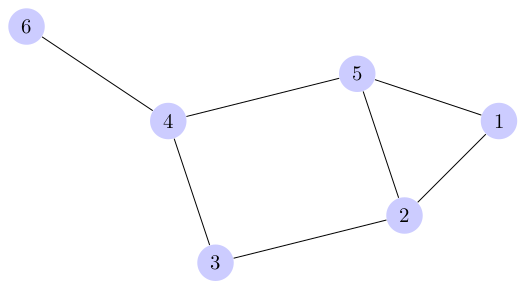
\includegraphics[width=0.85\linewidth]{figs/modeling-sums-continued-tikz01.png}
\end{center}

In an undirected graph, we do not distinguish the direction of the edge.  That is, for two vertices $i,j \in V$, we can equivalently write $(i,j)$ or $(j,i)$ to represent the edge.

\subsubsection{Directed Graphs}
Alternatively, we will want to consider directed graphs.  
\begin{definition}{}{}
A \emph{directed graph} (or di-graph for short) is denoted as $G = (V, A)$ where $V$ is a set of vertices and $A$ is a set of ordered pairs of vertices called arcs.  That is, an arc is like an edge, but the direction of it matters.
\end{definition}
For example, the following directed graph $G$ can be described by
\begin{itemize}
\item  the vertex set $V = \{1,2,3,4,5,6\}$ and 
\item the arc set $ A= \{(4,6),(6,4), (4,5), (5,1) (1,2), (2,5), (2,3), (3,4)\}$. 
\end{itemize}
\begin{center}
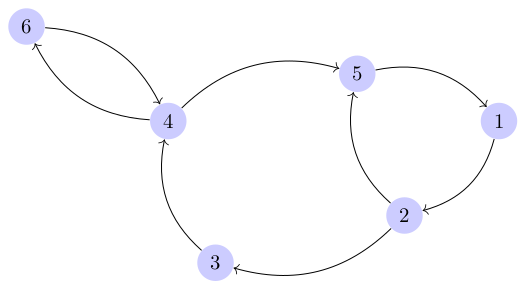
\includegraphics[width=0.85\linewidth]{figs/modeling-sums-continued-tikz02.png}
\end{center}

\subsection{Example: Minimum-Cost Flow in a Transportation Network}

\begin{examplewithallcode}{Minimum-Cost Network Flow}
{https://github.com/open-optimization/open-optimization-or-book/blob/master/Intro-Math-Programming/baseText/optimization/optimization-examples/network-flow-excel.xlsx}
{https://github.com/open-optimization/open-optimization-or-book/tree/master/Intro-Math-Programming/baseText/optimization/optimization-examples/network_flow_pulp.ipynb}
{https://github.com/open-optimization/open-optimization-or-book/tree/master/Intro-Math-Programming/baseText/optimization/optimization-examples/network_flow_gurobi.ipynb}

To illustrate the minimum-cost network flow problem, consider a company that wants to transport goods from two warehouses to two retail stores at the lowest possible cost. The company can send goods through a network of transportation routes, each with a given capacity and per-unit transportation cost.

The transportation network consists of:
\begin{itemize}
    \item \textbf{Two warehouses} (supply nodes) that store goods: 
          \begin{itemize}
              \item \textbf{Warehouse 1} can supply up to 20 units.
              \item \textbf{Warehouse 2} can supply up to 30 units.
          \end{itemize}
    \item \textbf{Two retail stores} (demand nodes) that require goods:
          \begin{itemize}
              \item \textbf{Store 1} requires 25 units.
              \item \textbf{Store 2} requires 25 units.
          \end{itemize}
    \item Transportation routes (\textbf{arcs}) connecting warehouses to stores, each with a transportation cost per unit and capacity limit.
\end{itemize}

\textbf{Graph Representation}

The transportation network can be represented as a directed graph \( G = (V, A) \), where:

\begin{itemize}
    \item \( V = \{ W_1, W_2, S_1, S_2 \} \) (two warehouses and two stores).
    \item \( A = \{(W_1, S_1), (W_1, S_2), (W_2, S_1), (W_2, S_2)\} \) (directed transportation routes).
    \item Each arc \( (i,j) \) has a given transportation cost \( C_{ij} \) and capacity \( u_{ij} \).
\end{itemize}

The network data is summarized in the following table:

    \begin{tabular}{|c|c|c|}
        \hline
        Route & Cost per unit ($c_{ij}$) & Capacity ($u_{ij}$) \\
        \hline
        Warehouse 1 to Store 1 & 4 & 15 \\
        Warehouse 1 to Store 2 & 6 & 10 \\
        Warehouse 2 to Store 1 & 5 & 20 \\
        Warehouse 2 to Store 2 & 2 & 20 \\
        \hline
    \end{tabular}

\modelhead{Model}

Let \( x_{ij} \) represent the amount of goods transported from warehouse \( i \) to store \( j \). The problem is formulated as:

\begin{align}
\min \quad & 4x_{W_1,S_1} + 6x_{W_1,S_2} + 5x_{W_2,S_1} + 2x_{W_2,S_2}\label{eq:example_objective} \\
    \st \quad
    & x_{W_1,S_1} + x_{W_1,S_2} \leq 20   \tag{Supply constraint for Warehouse 1}\label{eq:supply1} \\
    & x_{W_2,S_1} + x_{W_2,S_2} \leq 30   \tag{Supply constraint for Warehouse 2}\label{eq:supply2} \\
    & x_{W_1,S_1} + x_{W_2,S_1} = 25   \tag{Demand constraint for Store 1}\label{eq:demand1} \\
    & x_{W_1,S_2} + x_{W_2,S_2} = 25   \tag{Demand constraint for Store 2}\label{eq:demand2} \\
    & 0 \leq x_{ij} \leq u_{ij} &&\quad \text{for all } (i,j) \in A.\label{eq:capacity_constraint_example}
\end{align}

\textbf{Solution}

Solving the linear program, we obtain the following optimal flow values:

    \begin{tabular}{|c|c|}
        \hline
        Route & Optimal Flow ($x_{ij}$) \\
        \hline
        Warehouse 1 to Store 1 & 15 \\
        Warehouse 1 to Store 2 & 5 \\
        Warehouse 2 to Store 1 & 10 \\
        Warehouse 2 to Store 2 & 20 \\
        \hline
    \end{tabular}

The total minimum cost is given by:
\[
(4 \times 15) + (6 \times 5) + (5 \times 10) + (2 \times 20) = 60 + 30 + 50 + 40 = 180.
\]

\textbf{Interpretation of the Solution}

\begin{itemize}
    \item \textbf{Warehouse 1} sends \textbf{15 units} to Store 1 and \textbf{5 units} to Store 2.
    \item \textbf{Warehouse 2} sends \textbf{10 units} to Store 1 and \textbf{20 units} to Store 2.
    \item The \textbf{total transportation cost is minimized to 180}.
\end{itemize}

This solution meets all constraints while ensuring goods are transported at the lowest possible cost.

\end{examplewithallcode}
\newpage

\subsection{Minimum Cost Network Flow Problem}
\label{sec:min-cost-network-flow}

The \emph{minimum cost network flow problem} generalizes basic flow models by incorporating arc capacities, arc costs, and supply/demand at the nodes. The goal is to determine how to route flow through a network at the lowest possible cost while meeting demand and respecting all constraints.

\vspace{0.5em}
\noindent\textbf{Example: Amazonian's Distribution Network.}  
Amazonian must ship goods from large regional warehouses to local retail stores through intermediate distribution centers. Each warehouse has a certain supply capacity, each store has a demand, and each route incurs a transportation cost (fuel, time, and labor). Amazonian wants to decide how to route products to minimize cost, while ensuring demand is met and no transportation link exceeds its capacity.

\vspace{0.5em}
The figure below shows a small example. There are:
\begin{itemize}
\item Two warehouses (W1, W2) with a total of 50 units of supply,
\item Two distribution centers (D1, D2),
\item Three stores (S1, S2, S3) that need 20, 15, and 15 units, respectively,
\item Arc costs labeled in black,
\item Node demands/supplies shown in blue next to each node.
\end{itemize}

\vspace{-1em}
\begin{center}
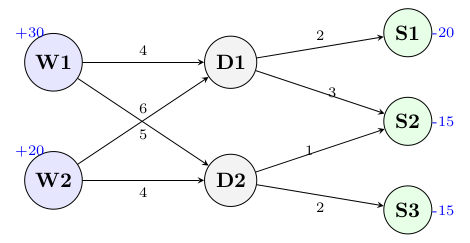
\includegraphics[width=0.85\linewidth]{figs/modeling-sums-continued-tikz03.png}
\end{center}

\noindent The problem is to determine how many units to send along each route to minimize the total shipping cost.

\smallskip \modelhead{Sets}
\begin{itemize}
\item \( V \): set of nodes in the network (warehouses, distribution centers, stores)
\item \( A \): set of directed arcs \( (i,j) \) representing shipment routes
\end{itemize}

\smallskip \modelhead{Parameters}
\begin{itemize}
\item \( c_{ij} \): cost per unit shipped on arc \( (i, j) \in A \)
\item \( u_{ij} \): maximum capacity of arc \( (i, j) \in A \)
\item \( d_i \): net demand at node \( i \in V \) (positive = demand, negative = supply)
\end{itemize}

\smallskip \modelhead{Variables} \\
\( x_{ij} \): amount of flow shipped along arc \( (i, j) \in A \)

\smallskip \modelhead{Model}
\begin{align*}
\min \quad & \sum_{(i,j) \in A} c_{ij} \cdot x_{ij} \\
\st \quad 
& \sum_{i : (i,k) \in A} x_{ik} - \sum_{j : (k,j) \in A} x_{kj} = d_k &&\quad \text{for all } k \in V   \tag{flow balance} \\
& 0 \leq x_{ij} \leq u_{ij} &&\quad \text{for all } (i,j) \in A   \tag{capacity constraints}
\end{align*}

\noindent This problem can be solved using linear programming, and efficient specialized algorithms exist due to its structure. Applications span:
\begin{itemize}
    \item Freight transportation,
    \item Supply chain optimization,
    \item Scheduling and telecommunications.
\end{itemize}

\subsection{(Unstructured) Minimum Cost Network Flow Problem}
The minimum cost network flow problem is an extension of the network flow problem that considers not only the capacities of the arcs, but also the costs associated with sending flow along the arcs and the demands at the nodes. The objective is to find the flow of minimum cost that satisfies the demands at the nodes and the capacity constraints on the arcs.

A network can be described as a directed graph \( G = (V, A) \), where \( V \) is the set of nodes and \( A \) is the set of arcs. Each arc \( (i, j) \in A \) has a capacity \( u_{ij} \) and a cost \( c_{ij} \). Each node \( i \in V\) has a demand \( d_i \), which can be positive, negative, or zero. A positive demand means that the node requires that amount of flow, a negative demand means that the node supplies that amount of flow, and a zero demand means that the node neither requires nor supplies flow.

Consider, for example:
The set of vertices is given by:
\[
V = \{ a, b, c, d, e, f, g, h \}
\]
The set of directed arcs is:
\[
A = \{ (b,a), (a,c), (b,d), (b,e), (c,e), (c,f), (h,d), (g,e), (e,h), (g,f) \}
\]
\begin{center}
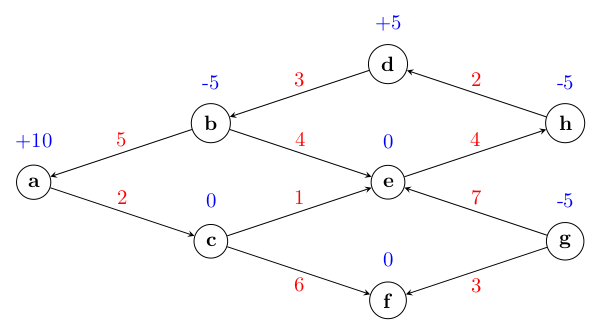
\includegraphics[width=0.85\linewidth]{figs/modeling-sums-continued-tikz04.png}
\end{center}
\begin{table}[h]
    \centering
    \begin{minipage}{0.45\textwidth}
        \centering
        \begin{tabular}{|c|c|c|}
            \hline
            \textbf{From} & \textbf{To} & \textbf{Cost} \\
            \hline
            b & a & {\color{red} 5 }\\
            a & c & {\color{red}2} \\
            d & b & {\color{red}3 }\\
            b & e & {\color{red}4 }\\
            c & e & {\color{red}1 }\\
            c & f & {\color{red}6 }\\
            h & d & {\color{red}2 }\\
            g & e & {\color{red}7 }\\
            e & h & {\color{red}4 }\\
            g & f & {\color{red}3} \\
            \hline
        \end{tabular}
        \caption{Arc Costs in the Network Flow Problem}
        \label{tab:arc_costs}
    \end{minipage}
    \hfill
    \begin{minipage}{0.45\textwidth}
        \centering
        \begin{tabular}{|c|c|}
            \hline
            \textbf{Node} & \textbf{Net Flow} \\
            \hline
            a & {\color{blue}+10} \\
            b & {\color{blue}-5} \\
            c & {\color{blue}0} \\
            d & {\color{blue}+5 }\\
            e & {\color{blue}0} \\
            f & {\color{blue}0} \\
            g & {\color{blue}-5} \\
            h & {\color{blue}-5} \\
            \hline
        \end{tabular}
        \caption{Net Flow at Each Node}
        \label{tab:net_flow}
    \end{minipage}
\end{table}
The minimum cost network flow problem can be defined as follows: Given a network \( G = (V, A) \), capacities \( u_{ij} \) and costs \( c_{ij} \) on the arcs, and demands \( d_i \) at the nodes, find the flow \( x_{ij} \) on the arcs that minimizes the total cost of the flow, while satisfying the demands at the nodes and the capacity constraints on the arcs.

\modelhead{Sets}
\begin{itemize}
\item \( V \): Set of nodes in the network.
\item \( A \): Set of arcs in the network.
\end{itemize}

\modelhead{Parameters}
\begin{itemize}
\item \( u_{ij} \): Capacity of arc \( (i, j) \in A \).
\item \( c_{ij} \): Cost per unit of flow on arc \( (i, j) \in A \).
\item \( d_i \): Change at node \( i \in V \).
\end{itemize}

\modelhead{Variables}
\begin{itemize}
\item \( x_{ij} \): Flow on arc \( (i, j) \in A \).
\end{itemize}

\modelhead{Model}
The minimum cost network flow problem can be formulated as a linear programming problem as follows:

\begin{align*}
\min \quad & \sum_{(i, j) \in A} c_{ij} x_{ij} \\
\st        & \sum_{i:(i, k) \in A} x_{ij} - \sum_{j:(k, j) \in A} x_{ji} = d_k &&\quad \text{for all } k \in V \\
& 0 \leq x_{ij} \leq u_{ij} &&\quad \text{for all } (i, j) \in A
\end{align*}

\modelhead{Objective}
- The objective is to minimize the total cost of the flow.

\modelhead{Constraints}
- Flow Conservation: The first set of constraints ensures that the flow into each node minus the flow out of the node is equal to the demand at the node.

- Capacity Constraints: The second set of constraints ensures that the flow on each arc does not exceed its capacity.

Minimum-cost network flow problems are widely used in transportation planning, supply chain logistics, and production scheduling, where the goal is to efficiently allocate resources at the lowest possible cost.

\subsection{Maximum flow}

The maximum flow problem is a fundamental problem in operations research and computer science, with applications in a wide variety of fields. It involves finding the maximum amount of flow that can be sent from a source node to a sink node in a network, without exceeding the capacities of the individual arcs, and ensuring that the flow on each arc is non-negative. This problem arises in many real-world situations, such as in transportation, where it can be used to find the maximum amount of goods that can be transported from a factory to a warehouse, or in telecommunications, where it can be used to find the maximum amount of data that can be sent from one server to another. Other applications include supply chain optimization, water distribution, and electrical power grid optimization. In this section, we will describe a linear programming formulation for the network flow problem.

A network can be described as a directed graph \( G = (V, A) \), where \( V \) is the set of nodes and \( A \) is the set of arcs. Each arc \( (i, j) \in A \) has a capacity \( u_{ij} \), which is the maximum amount of flow that can traverse the arc from node \( i \) to node \( j \).

The network flow problem can be defined as follows: Given a network \( G = (V, A) \), a source node \( s \), a sink node \( t \), and capacities \( u_{ij} \) on the arcs, find the maximum flow from \( s \) to \( t \) that respects the capacity constraints.

For example, consider the directed graph here with capacities on the arcs.
\begin{center}
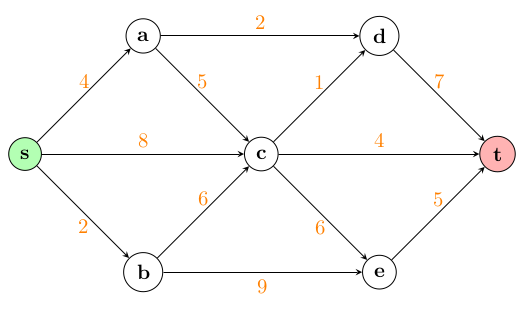
\includegraphics[width=0.85\linewidth]{figs/modeling-sums-continued-tikz05.png}
\end{center}

\begin{examplewithallcode}{Airline Transfer Network: Maximizing Passenger Throughput}
{https://github.com/open-optimization/open-optimization-or-book/blob/master/Intro-Math-Programming/baseText/optimization/optimization-examples/airline-maxflow-excel.xlsx}
{https://github.com/open-optimization/open-optimization-or-book/tree/master/Intro-Math-Programming/baseText/optimization/optimization-examples/airline_maxflow_pulp.ipynb}
{https://github.com/open-optimization/open-optimization-or-book/tree/master/Intro-Math-Programming/baseText/optimization/optimization-examples/airline_maxflow_gurobi.ipynb}
An airline is trying to reroute as many stranded passengers as possible from an origin city (\(s\)) to a destination city (\(t\)) using a network of connecting flights. Each flight has a known number of available seats, and passengers may transfer at intermediate airports. The objective is to determine the maximum number of passengers that can be routed from origin to destination, using available seat capacity and respecting flight routes.

\vspace{0.5em}
The network includes:
\begin{itemize}
    \item Origin airport \(s\),
    \item Intermediate hubs: \(a, b, c\),
    \item Regional transfer airports: \(d, e\),
    \item Final destination airport \(t\),
    \item Directed flight legs (arcs) with known seat availability.
\end{itemize}

\smallskip \modelhead{Sets and Parameters}
\begin{itemize}
    \item \( V = \{s, a, b, c, d, e, t\} \): set of airports.
    \item \( A = \{(s,a), (s,b), (s,c), (a,c), (a,d), (b,c), (b,e), (c,d), (c,e), (c,t), (d,e), (e,t)\} \): set of flight legs.
    \item \( u_{ij} \): number of available seats on flight from airport \( i \) to \( j \) for all $(i,j) \in A$.
\end{itemize}

\smallskip \modelhead{Variables} \\
\( x_{ij} \): number of passengers assigned to fly from airport \( i \) to \( j \) for all $(i,j) \in A$

\smallskip \modelhead{Model}
\begin{align*}
\max \quad & x_{sa} + x_{sb} + x_{sc} & \text{(max passengers from origin)} \\
\st \quad 
& x_{ac} + x_{ad} - x_{sa} = 0 & \text{(flow balance at \( a \))} \\
& x_{bc} + x_{be} - x_{sb} = 0 & \text{(at \( b \))} \\
& x_{cd} + x_{ce} + x_{ct} - x_{ac} - x_{bc} - x_{sc} = 0 & \text{(at \( c \))} \\
& x_{de} - x_{ad} - x_{cd} = 0 & \text{(at \( d \))} \\
& x_{et} - x_{be} - x_{ce} - x_{de} = 0 & \text{(at \( e \))} \\
& 0 \leq x_{sa} \leq 4,\quad 0 \leq x_{sb} \leq 2,\quad 0 \leq x_{sc} \leq 8 & \text{(available seats on initial flights)} \\
& 0 \leq x_{ac} \leq 5,\quad 0 \leq x_{ad} \leq 2,\quad 0 \leq x_{bc} \leq 6,\quad 0 \leq x_{be} \leq 9 \\
& 0 \leq x_{cd} \leq 1,\quad 0 \leq x_{ce} \leq 3,\quad 0 \leq x_{ct} \leq 4,\quad 0 \leq x_{de} \\
&\leq 7,\quad 0 \leq x_{et} \leq 5
\end{align*}
In compact summation notation form,  we have

$$
\begin{aligned}
\max \quad & \sum_{j \in V : (s,j) \in A} x_{sj} \\
\st        & \sum_{j \in V : (k,j) \in A} x_{kj} - \sum_{i \in V : (i,k) \in A} x_{ik} = 0 &&\quad \text{for all } k \in V \setminus \{s,t\} \\
           & 0 \leq x_{ij} \leq u_{ij} &&\quad \text{for all } (i,j) \in A
\end{aligned}
$$

\vspace{0.5em}
\noindent This model helps the airline determine how to assign passengers to flight legs in a way that makes maximum use of the network’s available capacity. It is especially useful during disruption scenarios like:
\begin{itemize}
    \item severe weather cancellations,
    \item emergency rerouting due to maintenance issues,
    \item high-demand events requiring temporary overflow routing.
\end{itemize}

The same framework can be extended to include priorities, time windows, or rebooking costs.
\end{examplewithallcode}

%
%
\begin{example}{}
\textbf{Sets and Parameters}
\begin{itemize}
\item \textbf{\underline{nodes}}: $V = \{s, a, b, c, d, e, t\}$
\item \textbf{\underline{arcs}}: $A = \{(s,a), (s,b), (s,c), (a,c), (a,d), (b,c), (b,e), (c,d), (c,e), (c,t), (d,e), (e,t)\}$
\item \textbf{\underline{capacities}}: $u_{ij}$ for each $(i,j) \in A$
\end{itemize}
%
\modelhead{Variables}
\begin{itemize}
\item \textbf{\underline{flow on arcs}}: $x_{ij}$ represents the flow on arc $(i,j) \in A$
\end{itemize}
%
%
\textbf{Explicit Model}
\begin{align*}
\max \quad & x_{sa} + x_{sb} + x_{sc} \\
\st \quad 
%    & x_{ac} + x_{bc} - x_{sa} - x_{sb} - x_{sc} = 0 \\
%    & x_{ad} + x_{cd} - x_{ac} = 0 \\
%    & x_{bc} + x_{be} + x_{ce} - x_{ac} = 0 \\
%    & x_{ct} + x_{et} - x_{ce} - x_{cd} = 0 \\
%    & x_{de} - x_{ad} - x_{cd} = 0 \\
%    & x_{et} - x_{de} - x_{be} = 0\\
%     &0 \leq x_{sa} \leq 4, \quad 0 \leq x_{sb} \leq 2, \quad 0 \leq x_{sc} \leq 8 \\
%    & 0 \leq x_{ac} \leq 5, \quad 0 \leq x_{ad} \leq 2, \quad 0 \leq x_{bc} \leq 6, \quad 0 \leq x_{be} \leq 9 \\
%    & 0 \leq x_{cd} \leq 1, \quad 0 \leq x_{ce} \leq 3, \quad 0 \leq x_{ct} \leq 4, \quad 0 \leq x_{de} \leq 7, \quad 0 \leq x_{et} \leq 5 \\
\end{align*}
%
\end{example}

The solution is shown here in bold values on the graph.  There is a total flow of 12.
\begin{center}
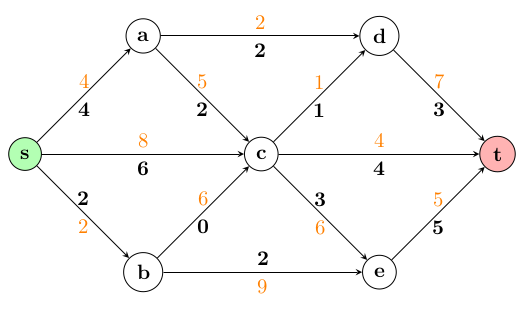
\includegraphics[width=0.85\linewidth]{figs/modeling-sums-continued-tikz06.png}
\end{center}

The maximum flow problem can be written mathematically in the following way.\\

\modelhead{Sets}
\begin{itemize}
\item \( V \): Set of nodes in the network.
\item \( A \): Set of arcs in the network.
\end{itemize}

\modelhead{Parameters}
\begin{itemize}
\item \( u_{ij} \): Capacity of arc \( (i, j) \in A \), which is the maximum amount of flow that can traverse the arc from node \( i \) to node \( j \).
\item \( s \): Source node.
\item \( t \): Sink node.
\end{itemize}

\modelhead{Variables}
\begin{itemize}
\item \( x_{ij} \): Flow on arc \( (i, j) \in A \).
\end{itemize}

\modelhead{Model}
The network flow problem can be formulated as a linear programming problem as follows:

\begin{align*}
\max \quad & \sum_{j:(s, j) \in A} x_{sj} \\
\st        & \sum_{i:(i, k) \in A} x_{ik} - \sum_{j:(k, j) \in A} x_{kj} = 0 &&\quad \text{for all } k \in V \setminus \{s, t\} \\
%& \sum_{j:(s, j) \in A} x_{sj} - \sum_{j:(j, s) \in A} x_{js} = \sum_{j:(j, t) \in A} x_{jt} - \sum_{j:(t, j) \in A} x_{tj} \\
& 0 \leq x_{ij} \leq u_{ij} &&\quad \text{for all } (i, j) \in A
\end{align*}

\modelhead{Objective}
- The objective is to maximize the total flow from the source node \( s \) to the sink node \( t \).

\modelhead{Constraints}
- Flow Balance: The first set of constraints ensures that the flow into each node is equal to the flow out of the node, except for the source and sink nodes.

- Capacity Constraints: The third set of constraints ensures that the flow on each arc does not exceed its capacity.

We will discuss duality later.  But duality is a concept that helps create bounds on a problem.
For this particular problem, we can think of a dual as a \emph{cut} in the graph - something that separates $s$ from $t$.  For example:
\begin{center}
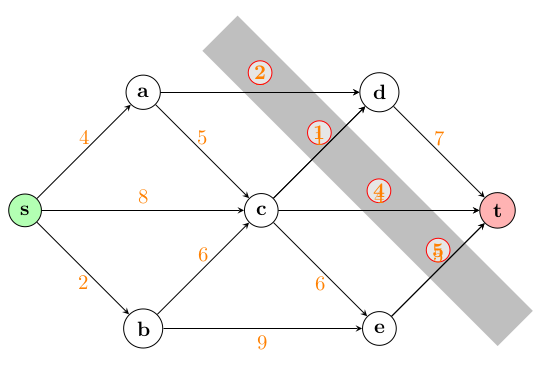
\includegraphics[width=0.85\linewidth]{figs/modeling-sums-continued-tikz07.png}
\end{center}
The selected arcs are a cut that separates $s$ from $t$.  The sum of their weights is $2 + 1 + 4 + 5 = 12$, which implies that there is not a flow more than 12 units from $s$ to $t$.

This bound is a form of \emph{duality}.  We will explore the concept more in later chapters.  This duality is captured in the following theorem.

\begin{theorem}{}
The maximum flow amount is equal to the size if the minimum cut.
\end{theorem}

%
%
\subsection{Multi-Commodity Minimum Cost Network Flow with Integrality Constraints}
\label{sec:multicommodity-flow}

The multi-commodity minimum cost network flow problem is a generalization of the minimum cost network flow problem that considers multiple commodities flowing through the network. Each commodity has its own demand at each node and its own cost on each arc. The objective is to find the integer flow of minimum cost that satisfies the demands of all commodities at the nodes and the capacity constraints on the arcs.

A network can be described as a directed graph \( G = (N, A) \), where \( N \) is the set of nodes and \( A \) is the set of arcs. Each arc \( (i, j) \in A \) has a capacity \( u_{ij} \). Each commodity \( k \) has a demand \( d_{ik} \) at each node \( i \in N \) and a cost \( c_{ijk} \) on each arc \( (i, j) \in A \).

The multi-commodity minimum cost network flow problem can be defined as follows: Given a network \( G = (N, A) \), capacities \( u_{ij} \) on the arcs, demands \( d_{ik} \) and costs \( c_{ijk} \) for each commodity \( k \), find the integer flow \( f_{ijk} \) on the arcs for each commodity \( k \) that minimizes the total cost of the flow, while satisfying the demands of all commodities at the nodes and the capacity constraints on the arcs.

\modelhead{Sets}
\begin{itemize}
\item \( N \): Set of nodes in the network.
\item \( A \): Set of arcs in the network.
\item \( K \): Set of commodities.
\end{itemize}
%
\modelhead{Parameters}
\begin{itemize}
\item \( u_{ij} \): Capacity of arc \( (i, j) \in A \).
\item \( c_{ijk} \): Cost per unit of flow of commodity \( k \) on arc \( (i, j) \in A \).
\item \( d_{ik} \): Demand of commodity \( k \) at node \( i \in N \).
\end{itemize}
%
\modelhead{Variables}
\begin{itemize}
\item \( f_{ijk} \): Flow of commodity \( k \) on arc \( (i, j) \in A \).
\end{itemize}
%
\modelhead{Model}
The multi-commodity minimum cost network flow problem can be formulated as an integer linear programming problem as follows:

\begin{align*}
\min \quad & \sum_{k \in K} \sum_{(i, j) \in A} c_{ijk} f_{ijk} \\
\st        & \sum_{k \in K} \left( \sum_{j:(i, j) \in A} f_{ijk} \right) \leq u_{ij} &&\quad \text{for all } (i, j) \in A \\
& \sum_{j:(i, j) \in A} f_{ijk} - \sum_{j:(j, i) \in A} f_{jik} = d_{ik} &&\quad \text{for all } i \in N, \; \forall k \in K \\
& f_{ijk} \in \mathbb{Z}_{\geq 0} &&\quad \text{for all } (i, j) \in A, \; \forall k \in K
\end{align*}

\modelhead{Objective}
The objective is to minimize the total cost of the flow, summed over all commodities and all arcs.

\modelhead{Constraints}
\begin{itemize}
\item \textbf{Capacity Constraints:} The first set of constraints ensures that the total flow on each arc (summed across all commodities) does not exceed its capacity.
\item \textbf{Flow Conservation:} The second set of constraints ensures that, for each commodity, the net flow into each node equals the demand of that commodity at the node.
\item \textbf{Integrality Constraints:} The third set of constraints ensures that the flow on each arc for each commodity is a non-negative integer.
\end{itemize}


\begin{examplewithallcode}{Multi-commodity network flow}
{}
{https://github.com/open-optimization/open-optimization-or-book/tree/master/Intro-Math-Programming/baseText/optimization/optimization-examples/multicommodity_flow_pulp.ipynb}
{https://github.com/open-optimization/open-optimization-or-book/tree/master/Intro-Math-Programming/baseText/optimization/optimization-examples/multicommodity_flow_gurobi.ipynb}
\label{ex:multicommodity-network-flow}

Consider a small network with 4 nodes and 4 arcs, transporting 2 commodities. Each arc has a shared capacity, and each commodity has its own per-unit cost on each arc and its own supply/demand pattern at the nodes (negative values indicate supply, positive values indicate demand).
\begin{verbatim}
# Sample data
nodes = [1, 2, 3, 4]
arcs = [(1, 2), (1, 3), (2, 4), (3, 4)]
commodities = [1, 2]
capacities = {(1, 2): 20, (1, 3): 15, (2, 4): 25, (3, 4): 20}
costs = {(1, 2, 1): 2, (1, 2, 2): 3, (1, 3, 1): 3,
         (1, 3, 2): 2, (2, 4, 1): 1, (2, 4, 2): 2,
         (3, 4, 1): 2, (3, 4, 2): 1}
demands = {(1, 1): -10, (1, 2): -5, (2, 1): 0, (2, 2): 0,
           (3, 1): 0,   (3, 2): 0,  (4, 1): 10, (4, 2): 5}
\end{verbatim}

The two figures below show the input network (left) and the optimal flow assignment (right). Each arc is labelled with the commodity flows it carries; the arc capacity constraint requires the sum of those commodity flows to stay within the arc's capacity.

% --- TikZ recreation of networkx figure: multi-network-flow-data.png ---
% Non-floating (this block sits inside the framed examplewithallcode box,
% which cannot contain figure/table floats).
\begin{center}
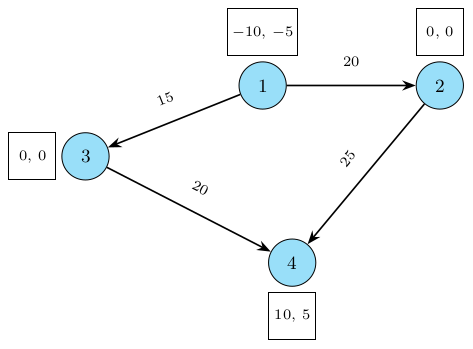
\includegraphics[width=0.85\linewidth]{figs/modeling-sums-continued-tikz08.png}
\captionof{figure}{Data for multi-commodity network flow example: four nodes with paired supplies/demands $(d_{i1}, d_{i2})$ and four arcs labelled with their shared capacities.}
\label{fig:multi-network-flow-data.png}
\end{center}

% --- TikZ recreation of networkx figure: multi-network-flow-solution.png ---
\begin{center}
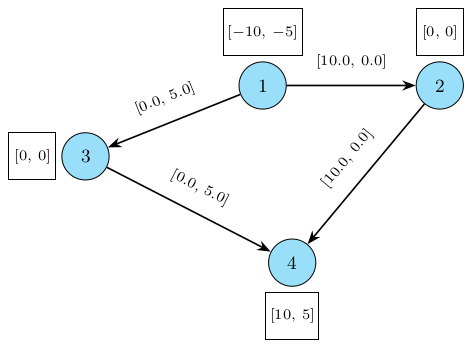
\includegraphics[width=0.85\linewidth]{figs/modeling-sums-continued-tikz09.png}
\captionof{figure}{Solution to multi-commodity network flow: each arc is labelled with the optimal flow of each commodity $[f_{ij1}, f_{ij2}]$.}
\label{fig:multi-network-flow-solution.png}
\end{center}

\end{examplewithallcode}
%
\subsection{Multicommodity Flow: Source--Sink Formulation}
\label{sec:multicommodity-source-sink}

A common alternative formulation of the multi-commodity flow problem expresses each commodity in terms of a single source node, a single sink node, and a demand value, with flow variables that represent the fraction of the demand routed on each arc. The formulation below follows the description on the Wikipedia article \url{https://en.wikipedia.org/wiki/Multi-commodity_flow_problem}.

\paragraph{Problem Definition}
Given a flow network \(G(V,E)\), where each edge \((u,v) \in E\) has capacity \(c(u,v)\), suppose there are \(k\) commodities
\(K_1,K_2,\dots,K_k\), defined by \(K_i=(s_i,t_i,d_i)\), where \(s_i\) and \(t_i\) are the \textbf{source} and \textbf{sink} of commodity \(i\), and \(d_i\) is its demand. The variable \(f_i(u,v)\) denotes the fraction of commodity \(i\) routed along edge \((u,v)\); we take \(f_i(u,v) \in [0,1]\) when flow may be split among multiple paths, and \(f_i(u,v) \in \{0,1\}\) when each commodity must follow a single path (``single path routing''). The problem is to find an assignment of all flow variables that satisfies the following four conditions.

\textbf{(1) Link capacity.} The total flow routed over any link, weighted by demands, does not exceed the link's capacity:
\[
\forall (u,v)\in E:\quad \sum_{i=1}^{k} f_i(u,v)\cdot d_i \;\leq\; c(u,v).
\]

\textbf{(2) Flow conservation on transit nodes.} For any intermediate node \(u\) (other than the source or sink of commodity \(i\)), the flow of commodity \(i\) entering \(u\) equals the flow leaving \(u\):
\[
\sum_{w \in V} f_i(u,w) - \sum_{w \in V} f_i(w,u) \;=\; 0 \quad \text{whenever } u \neq s_i, t_i.
\]

\textbf{(3) Flow conservation at the source.} The full unit of commodity \(i\) must leave its source:
\[
\sum_{w \in V} f_i(s_i,w) - \sum_{w \in V} f_i(w,s_i) \;=\; 1.
\]

\textbf{(4) Flow conservation at the destination.} The full unit of commodity \(i\) must arrive at its sink:
\[
\sum_{w \in V} f_i(w,t_i) - \sum_{w \in V} f_i(t_i,w) \;=\; 1.
\]

\paragraph{Corresponding optimization problems.}
Three natural objective functions can be paired with the constraints above:
\begin{itemize}
\item \textbf{Load balancing} minimizes the variation in link utilization \(U(u,v) = \tfrac{\sum_{i=1}^{k} f_i(u,v) \cdot d_i}{c(u,v)}\); a common linearization is to minimize the maximum utilization \(U_{\max}\) subject to \(U_{\max} \geq U(u,v)\) for every arc.
\item \textbf{Minimum cost multi-commodity flow} attaches a per-unit cost \(a(u,v)\) to each arc and minimizes \(\sum_{(u,v)\in E} a(u,v) \sum_{i=1}^{k} f_i(u,v) \cdot d_i\).
\item \textbf{Maximum multi-commodity flow} leaves the demands \(d_i\) variable and maximizes the total throughput \(\sum_{i=1}^{k} d_i\).
\end{itemize}

\paragraph{Relation to other problems.}
The minimum-cost variant generalizes the (single-commodity) minimum cost flow problem of Section~\ref{sec:min-cost-network-flow} (which has only one source \(s\) and one sink \(t\)). More broadly, every flow problem can be cast as a special case of the \emph{circulation problem}.

\begin{examplewithallcode}{Source--Sink Multicommodity Flow}
{}
{https://github.com/open-optimization/open-optimization-or-book/tree/master/Intro-Math-Programming/baseText/optimization/optimization-examples/multicommodity_sourcesink_pulp.ipynb}
{https://github.com/open-optimization/open-optimization-or-book/tree/master/Intro-Math-Programming/baseText/optimization/optimization-examples/multicommodity_sourcesink_gurobi.ipynb}
Consider the directed network on nodes \(V=\{1,2,3,4\}\) with the arc capacities \(c(u,v)\) and per-unit costs \(a(u,v)\) listed below. Two commodities must be routed from source node \(1\) to sink node \(4\): commodity~1 with demand \(d_1=10\) and commodity~2 with demand \(d_2=5\).

\begin{center}
\begin{tabular}{c|c|c}
Arc \((u,v)\) & Capacity \(c(u,v)\) & Cost \(a(u,v)\) \\
\hline
\((1,2)\) & 10 & 1 \\
\((1,3)\) &  8 & 2 \\
\((2,3)\) &  4 & 1 \\
\((2,4)\) &  7 & 3 \\
\((3,4)\) &  9 & 1 \\
\end{tabular}
\end{center}

Using the fractional flow variables \(f_i(u,v)\in[0,1]\) with the minimum-cost objective and constraints (1)--(4), the optimal routing sends all of commodity~2 along \(1\to 3\to 4\) and splits commodity~1 across the \(1\to 2\to 4\) and \(1\to 3\to 4\) paths (routing a small share through arc \((2,3)\)), for a minimum total cost of \(\mathbf{51}\).
\end{examplewithallcode}

\section{Transportation Problem}
\label{sec:transportation-problem}

The transportation problem involves determining the optimal way to transport goods from a set of suppliers to a set of markets. The goal is to minimize total transportation costs while satisfying supply availabilities at the suppliers and demand requirements at the markets.

\noindent Additional resources:
\begin{itemize}
\item \href{https://www.youtube.com/watch?v=Jr7LI-sUEmo}{YouTube: Transportation problem with PuLP in Python}
\item \href{https://nbviewer.jupyter.org/github/Pyomo/PyomoGallery/blob/master/transport/transport.ipynb}{Notebook: Solution with Pyomo}
\end{itemize}

Let $I$ be the set of suppliers and $J$ be the set of markets.

\modelhead{Parameters}
\begin{itemize}
\item $s_i$: supply available at supplier $i$
\item $d_j$: demand required at market $j$
\item $c_{ij}$: cost of shipping one unit from supplier $i$ to market $j$
\end{itemize}

\modelhead{Variables}
\begin{itemize}
\item $x_{ij}$: units shipped from supplier $i$ to market $j$
\end{itemize}

\modelhead{Model}
\begin{align*}
\text{minimize:} \quad &\sum_{i\in I}\sum_{j \in J} c_{ij}\,x_{ij} && \text{(total shipping cost)}\\
\text{subject to:} \quad &\sum_{j\in J} x_{ij} \leq s_i && \forall i \in I && \text{(supply limit at each supplier)}\\
&\sum_{i\in I} x_{ij} = d_j && \forall j \in J && \text{(demand met at each market)}\\
& x_{ij} \geq 0 && \forall i\in I,\; j\in J && \text{(non-negativity)}
\end{align*}

The objective minimizes total shipping cost; the constraints ensure that the shipment from each supplier does not exceed its available supply, and that the demand at each market is satisfied. The decision variables $x_{ij}$ specify the optimal shipment quantities.

\section*{Concluding Comments}

\subsection*{Solving the Minimum-Cost Network Flow Problem}
This problem can be efficiently solved using specialized algorithms such as:
\begin{itemize}
\item \textbf{Successive Shortest Path Algorithm}: Iteratively sends flow along the shortest-cost paths.
\item \textbf{Cycle-Canceling Algorithm}: Identifies negative-cost cycles and eliminates them to reach optimality.
\item \textbf{Network Simplex Method}: An adaptation of the simplex method designed specifically for network flow problems.
\item \textbf{Linear Programming Solvers}: General-purpose solvers such as the Simplex or Interior-Point methods can handle large instances.
\end{itemize}

\begin{resource}
%Other examples:
\begin{itemize}
\item \href{https://gurobi.github.io/modeling-examples/food_manufacturing_1_2/food_manufacture_1.html}{Food manfacturing - GUROBI}
\item \href{https://www.andrew.cmu.edu/user/gc0v/webpub/book.pdf}{Optimization Methods in Finance - Corneujols, T\"ut\"unc\"u}
\end{itemize}
\end{resource}
%
%
\section{Multi-Period Capital Investment}
\label{sec:multi-period-capital-investment}

\begin{examplewithallcode}{Multi-Period Capital Investment Problem}
{https://github.com/open-optimization/open-optimization-or-book/blob/master/Intro-Math-Programming/baseText/optimization/optimization-examples/multi-period-investment-excel.xlsx}
{https://github.com/open-optimization/open-optimization-or-book/tree/master/Intro-Math-Programming/baseText/optimization/optimization-examples/multi_period_investment_pulp.ipynb}
{https://github.com/open-optimization/open-optimization-or-book/tree/master/Intro-Math-Programming/baseText/optimization/optimization-examples/multi_period_investment_gurobi.ipynb}
\label{ex:multi-period-capital-investment}

You are managing a multi-period investment fund with \$50,000 to start. Over the course of four periods, you can allocate capital to a set of investment opportunities. Each investment requires an upfront cost and offers an expected payout at the beginning of the following period, which can then be reinvested. The goal is to maximize the total funds available at the end of the fourth period.

The following table lists the available investments, the required initial investment for each period, and their respective payouts for the next period. Formulate an LP to determine the optimal investment strategy over the four periods.

\end{examplewithallcode}

\begin{table}[h!]
\begin{center}
\begin{tabular} {|c|l|r|r|}
\hline
Period & Investment & Investment Required (\$) & Payout in Next Period (\$) \\
\hline\hline
1 & A & 10{,}000 & 15{,}000 \\
1 & B & 20{,}000 & 30{,}000 \\
1 & C & 15{,}000 & 22{,}000 \\
\hline
2 & D & 12{,}000 & 18{,}000 \\
2 & E & 25{,}000 & 35{,}000 \\
2 & F & 18{,}000 & 26{,}000 \\
\hline
3 & G & 15{,}000 & 20{,}000 \\
3 & H & 10{,}000 & 14{,}000 \\
3 & I & 20{,}000 & 28{,}000 \\
\hline
4 & J &  8{,}000 & 10{,}000 \\
4 & K & 16{,}000 & 22{,}000 \\
4 & L & 12{,}000 & 16{,}000 \\
\hline
\end{tabular}
\caption{Investment Opportunities Over Four Periods}
\label{tab:multi_period_investments}
\end{center}
\end{table}

\begin{solution}

\modelhead{Variables} \\
$x_{i,t}$: whether to invest in opportunity $i$ during period $t$, where $x_{i,t} = 1$ if investment $i$ is chosen in period $t$, and $x_{i,t} = 0$ otherwise.

\modelhead{Parameters} \\
$c_{i,t}$: investment required for opportunity $i$ in period $t$. \\
$p_{i,t}$: payout from investment $i$ in the next period.

\smallskip \modelhead{Objective} The cash on hand at the end of period 4 is the payout of the period-4 investments:
\[
\max \quad z = 10{,}000\,x_{J} + 22{,}000\,x_{K} + 16{,}000\,x_{L}.
\]

\smallskip \modelhead{Constraints}
\begin{itemize}
\item \textbf{Period 1 budget constraint:}
\[
10{,}000\,x_A + 20{,}000\,x_B + 15{,}000\,x_C \;\leq\; 50{,}000.
\]
\item \textbf{Period 2 budget constraint:}
\[
12{,}000\,x_D + 25{,}000\,x_E + 18{,}000\,x_F \;\leq\; 15{,}000\,x_A + 30{,}000\,x_B + 22{,}000\,x_C.
\]
\item \textbf{Period 3 budget constraint:}
\[
15{,}000\,x_G + 10{,}000\,x_H + 20{,}000\,x_I \;\leq\; 18{,}000\,x_D + 35{,}000\,x_E + 26{,}000\,x_F.
\]
\item \textbf{Period 4 budget constraint:}
\[
8{,}000\,x_J + 16{,}000\,x_K + 12{,}000\,x_L \;\leq\; 20{,}000\,x_G + 14{,}000\,x_H + 28{,}000\,x_I.
\]
\item \textbf{Binary decision variables:}
\[
x_{i,t} \in \{0,1\}, \quad \forall i,\; \forall t.
\]
\end{itemize}

% TODO(author): the 0--1 formulation above assumes each investment opportunity
% can be chosen at most once. Consider whether a continuous (LP) formulation
% with $x_{i,t} \in [0,1]$ or an unbounded investment level would be preferred
% for this example, and add the resulting numerical solution / interpretation.

\end{solution}

\section{Exercises}
\begin{ex}{\textbf{Fair Housing Assignment for 12 Families:}}{}

A new apartment complex has been completed, and 12 families need to be assigned to 12 available apartments. Each family has ranked the apartments (1 = most preferred, 12 = least preferred). 
\begin{enumerate}
\item Use Excel Solver to find an assignment that minimizes the sum of preferences.

\item What units were assigned to which families, and what was their preference score?

\item What is the worst preference score assigned?
\end{enumerate}
Download the data for this problem here \href{https://github.com/open-optimization/open-optimization-or-book/blob/master/Intro-Math-Programming/baseText/optimization/optimization-examples/Family-Apartment_Preferences__12_.csv}{data}.
\end{ex}
\begin{ex}\textbf{Maximum Network Flow to a Single Node} 
{}{}
A disaster relief effort is underway to transport supplies to a central distribution hub in a flooded region. The network consists of multiple warehouses (nodes) that currently have varying inventory levels of emergency supplies. Each transportation route (arc) between warehouses is serviced by a single truck with a limited carrying capacity. The goal is to determine the optimal transportation plan that maximizes the amount of supplies delivered to the central hub while respecting inventory constraints and truck capacities on each route.

Formulate a max-flow optimization problem for this scenario. Define your decision variables, objective function, and constraints explicitly.  Assume that you do not want to leave any inventory at the distribution centers.

    \begin{tabular}{|c|c|c|c|c|}
        \hline
        \textbf{Node} & \textbf{Type} & \textbf{Inventory (if applicable)} & \textbf{Connected To} & \textbf{Capacity} \\
        \hline
        W1 & Warehouse & \textbf{200} & D1 & 100 \\
        W2 & Warehouse & \textbf{300} & D1 & 150 \\
        W3 & Warehouse & \textbf{150} & D2 & 120 \\
        W4 & Warehouse & \textbf{250} & D3 & 100 \\
        W5 & Warehouse & \textbf{180} & D3 & 90 \\
        \hline
        D1 & Distribution  & N/A & Hub, D2 & 200, 80 \\
        D2 & Distribution & N/A & Hub & 180 \\
        \hline
        Hub & Central Hub & N/A & D3 & 160 \\
        \hline
        D3 & Distribution & N/A & W4, W5 & 100, 90 \\
        \hline
    \end{tabular}
    
\begin{center}
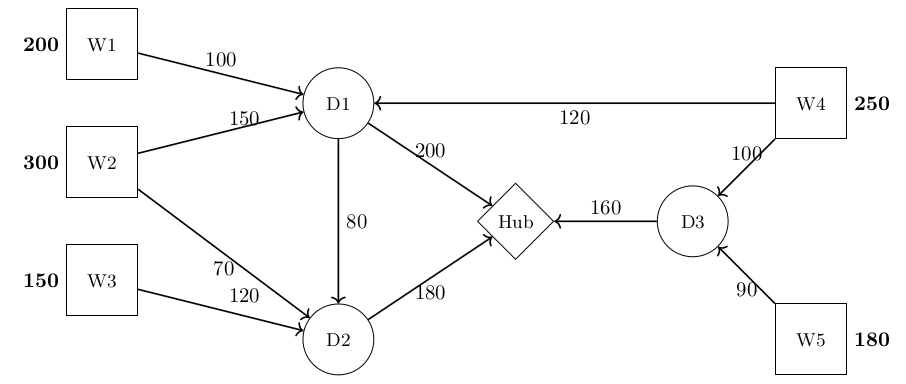
\includegraphics[width=0.85\linewidth]{figs/modeling-sums-continued-tikz10.png}
\end{center}

\end{ex}

\begin{ex}\textbf{Max flow.}{}

Write out the explicit constraints that define the max flow problem given in the picture.  
Solve this problem as a linear program using Excel.

\begin{center}
    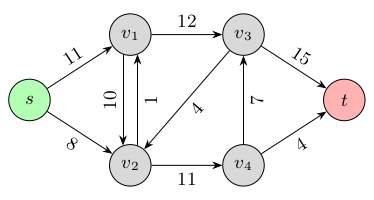
\includegraphics[width=0.85\linewidth]{figs/modeling-sums-continued-tikz11.png}
%\end{document} % removed: this was prematurely ending the document
\end{center}
\end{ex}

\begin{ex}{Min Cost Network Flow}{}
Use the picture below to formulate the corresponding capacitated min cost network flow.  Solve this problem using Excel.  

\begin{center}
    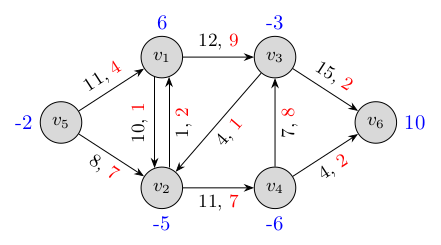
\includegraphics[width=0.85\linewidth]{figs/modeling-sums-continued-tikz12.png}
   \end{center}
   \end{ex}

% NOTE (2026-07-08): Two TikZ figures recreated from old networkx PNGs
% (network-flow.png / network-flow-solution.png) were removed here.  They were
% unreferenced leftovers (commented out in earlier versions), matched no example
% or exercise in the chapter, and the inferred solution values violated flow
% conservation at nodes 4 and 5.  If a worked min-cost-flow example is wanted
% here, regenerate the figures from actual solver output.  The TikZ code is in
% git history at commit 8c97ba9 (lines 1219-1278).


